\documentclass{report}
\usepackage[utf8]{inputenc}
\usepackage[italian]{babel}

\usepackage{amsmath}
\usepackage{amssymb}
\usepackage{amsthm}
\usepackage{mathtools}

\usepackage{float}
\usepackage{graphicx}
\graphicspath{ {images/} }
\usepackage{microtype}

\usepackage[margin=1in]{geometry}
\usepackage[default]{lato}
\usepackage[T1]{fontenc}

\setlength{\parindent}{0pt}

\theoremstyle{theorem}
\newtheorem*{definition}{Definizione}
\theoremstyle{theorem}
\newtheorem*{property}{Proprietà}
\theoremstyle{theorem}
\newtheorem*{theorem}{Teorema}
\theoremstyle{theorem}
\newtheorem*{example}{Esempio}

\newcommand*\dif{\mathop{}\!\mathrm{d}}

\title{Complementi di Matematica}
\author{Cristian Baldi}
\date{2015/2016}

\begin{document}

\maketitle
\tableofcontents

\chapter{Matrici}

\section{Definizione}

Una matrice con $p$ righe e $q$ colonne è una tabella di numeri reali così disposti:

$$
A =
\begin{bmatrix}
    a_{1,1} & a_{1,2} & a_{1,3} & \dots  & a_{1,q} \\
    a_{2,1} & a_{2,2} & a_{2,3} & \dots  & a_{2,q} \\
    \vdots & \vdots & \vdots & \ddots & \vdots \\
    a_{p,1} & a_{p,2} & a_{p,3} & \dots  & a_{p,q}
\end{bmatrix}
$$

I parametri $p$ e $q$ sono detti dimensioni della matrice.

L'elemento $A_{i,j}$ della matrice è l'elemento che si trova alla $i$-esima riga e alla $j$-esima colonna.

\section{Matrici quadrate}

Una matrice che ha dimensione $(n,n)$ è detta matrice quadrata. Questa matrice avrà un numero uguale di righe e di colonne.

$$
A_{\text{quadrata 2x2}} =
\begin{bmatrix}
    a_{1,1} & a_{1,2} \\
    a_{2,1} & a_{2,2}
\end{bmatrix}
$$

\section{Diagonale principale}

Per ogni matrice quadrata $A_{n \times n}$ è possibile individuare gli elementi della diagonale principale, cioè tutti gli $a_{i,i}$ con $i$ che varia da 1 a $n$.

\section{Matrice triangolare superiore}

Una matrice quadrata $A_{n\times n}$ si dice triangolare superiore se tutti gli elementi che si trovano sotto la diagonale principale sono nulli.

\[
A_{\text{Diag. Sup.}} =
\begin{bmatrix}
    1 & 2 & 3 \\
    0 & 4 & 5 \\
    0 & 0 & 6 \\
\end{bmatrix}
\]

\section{Matrice diagonale}

Una matrice quadrata $A_{n \times n}$ è detta diagonale se tutti gli elementi non appartenenti alla diagonale principale sono nulli.

\section{Matrice simmetrica}

Una matrice quadrata si dice simmetrica se i suoi elementi in posizioni simmetriche rispetto alla diagonale principale sono uguali.

\section{Matrice identità}

Chiamiamo matrice unità (o matrice identica o matrice identità) di ordine $n$ la matrice quadrata $I_{n \times n}$ avente tutti gli elementi della diagonale principale uguali a 1 e tutti gli altri elementi uguali a 0.

La matrice identica è una matrice diagonale.

\section{Operazioni con matrici}

\subsection{Matrice trasposta}

Presa una matrice $A$ chiamiamo $A^t$ la trasposta di $A$ la
matrice avente come elemento di posto $(i, j)$ l'elemento $(j, i)$
della matrice A.

$$
A =
\begin{bmatrix}
    1 & 2 & 3\\
    4 & 5 & 6
\end{bmatrix}
$$

$$
A^t =
\begin{bmatrix}
    1 & 4 \\
    2 & 5 \\
    3 & 6
\end{bmatrix}
$$

\subsection{Somma tra matrici}

Consideriamo due matrici $A$ e $B$. Le due matrici sono sommabili se
e solo se sono dello stesso tipo, cioè se e solo se hanno lo stesso
numero di righe e di colonne.

$C=A+B$ è una matrice avente lo stesso numero di righe e di colonne
delle due matrici di partenza, in cui ogni termine
$C_{i,j}=A_{i,j}+B_{i,j}$.

$$
A =
    \begin{bmatrix}
    2 & 5 & -3 \\
    1 & -2 & 4
    \end{bmatrix}
$$

$$
B =
    \begin{bmatrix}
    7 & -5 & 2 \\
    -9 & 4 & -1
    \end{bmatrix}
$$

$$
C = A+B = \begin{bmatrix}
    2+7 & 5+(-5) & (-3)+2 \\
    (-9)+1 & (-2)+4 & 4+(-1)
    \end{bmatrix}
    =
    \begin{bmatrix}
    9 & 0 & -1 \\
    -8 & 2 & 3
    \end{bmatrix}
$$

\subsection{Moltiplicazione per uno scalare}

La moltiplicazione di una matrice $A=(a_{i,j})$ per uno scalare $r$ è ottenuta moltiplicando ogni elemento di $A$ per lo scalare stesso.
$$ rA = (ra_{i,j}) $$

\subsection{Prodotto tra matrici}

\begin{definition}
Siano $A, B$ due matrici. E' possibile calcolare il prodotto $C=A \cdot B$
solo se $righe(A) = colonne(B)$ e $colonne(A) = righe(B)$.
\end{definition}

$$C_{ij} := A_{i1} \cdot B_{1j} + A_{i2} \cdot B_{2j} + \ldots + A_{iq} \cdot B_{qj}$$

\subsection{Inversa di una matrice}

\begin{theorem}
Una matrice è invertibile se e solo se ha rango massimo.
\end{theorem}

Quindi una matrice ammette inversa se il $det(A) \neq 0$

\begin{theorem}
Sia $A$ una matrice quadrata di ordine $n$. Se è invertibile è possibile calcolare $A^{-1}=(x_{ij})$ in questo modo:
$$ x_{ij} = \frac{(-1)^{i+j}\cdot det(A_{ji})}{det(A)}$$

dove $A_{ij}$ è la matrice ottenuta eliminando da $A$ la riga $i$-esima e la colonna $j$-esima.
\end{theorem}

\section{Rango}

\begin{definition}
Il rango di una matrice è il massimo ordine di sottomatrice quadrata con determinante diverso da 0 che posso estrarre dalla matrice stessa.
\end{definition}

\begin{definition}
Il rango di una matrice ridotta a scala è il numero di righe diverse da 0.
\end{definition}

Una matrice rettangolare $A_{m \times n}$ può avere rango al massimo uguale al minimo tra il numero di righe e il numero di colonne della matrice. Cioè:
$$rk(A)\leq min(m,n)$$

Nel caso in cui il rango coincida con il minimo tra $m$ ed $n$, cioè $rk(A)= min(m,n)$, diremo che la matrice ha rango massimo.

\section{Riduzione a scala}

\begin{definition}
Una matrice $A$ si dice a scala se il numero degli zeri che precede il primo elemento diverso da zero di ogni riga aumenta precedendo dalla prima riga verso l'ultima, fino a che non restano, eventualmente, solo righe nulle.
\end{definition}

\section{Determinante}

\begin{definition}
Il determinante è un numero associato ad una matrice $A$ e si indica come $|A|$ oppure con $det(A)$.
\end{definition}

\subsection{Calcolare il determinante}

\subsubsection{Matrice 2$\times$2}

$$A=\left[\begin{matrix}a & b\\ c & d\end{matrix}\right] \rightarrow det(A) = a \cdot d - b \cdot c$$

\subsubsection{Matrice 3$\times$3}

Attraverso la regola di Sarrus

$$A=\left[\begin{matrix}a_{11} & a_{12} & a_{13}\\ a_{21} & a_{22} & a_{23}\\ a_{31} & a_{32} & a_{33}\end{matrix}\right]$$

$$det(A)=(a_{11}a_{22}a_{33}+a_{12}a_{23}a_{31}+a_{13}a_{21}a_{32})-(a_{31}a_{22}a_{13}+a_{32}a_{23}a_{11}+a_{21}a_{12}a_{33})$$

\subsubsection{Matrici n$\times$n}

Consideriamo una matrice quadrata di ordine $n$

$$A=\left[\begin{matrix} a_{11} & a_{12}& \dots& a_{1n} \\ a_{21} & a_{22}& \dots &a_{2n}\\ \vdots & \ddots &\ddots & \vdots\\ a_{n1}& a_{n2} & \dots & a_{nn} \end{matrix}\right]$$

e denotiamo con $A_{ij}$ la matrice che si ottiene eliminando dalla matrice $A$ la riga $i$ e la colonna $j$.

\begin{definition}{Sviluppo di Laplace per righe}
    $$det(A)=\sum_{j=1}^n{(-1)^{i+j}a_{ij}det(A_{ij})}$$
    (ci si muove lungo la riga i-esima).
\end{definition}

\begin{definition}{Sviluppo di Laplace per colonne}
    $$det(A)=\sum_{i=1}^n{(-1)^{i+j}a_{ij}det(A_{ij})}$$
    (ci si muove lungo la colonna j-esima).
\end{definition}

\subsection{Proprietà determinante}

\begin{property}
    Una matrice quadrata con due righe o due colonne uguali ha determinante nullo.
\end{property}

\begin{property}
    Siano $A$ e $B$ due matrici quadrate di ordine $n$ che si ottengono una dall'altra scambiando fra loro due righe. Allora $det(A) = -det(B)$. Un'analoga proprietà vale per lo scambio di colonne.
\end{property}

\begin{property}
    Se una matrice quadrata $A$ ha una riga che è multipla di un'altra, allora $det(A)=0$. Un'analoga proprietà vale per le colonne.
\end{property}

\begin{property}
    Sia $A$ una matrice quadrata di ordine $n$ e $k$ un numero reale. Si ha allora: $$det (kA) = k^n \det A$$
\end{property}

\begin{property}
    Sia $A$ una matrice diagonale, allora il determinante è uguale al prodotto degli elementi della diagonale.
\end{property}

\begin{theorem}[di Binet]
    Date due matrici quadrate dello stesso $A$ e $B$ si ha: $$ det(AB) = \det A \det B$$
\end{theorem}

\begin{theorem}
    Se $A$ è una matrice invertibile allora $det(A^{-1}) = \frac{1}{det(A)}$.
\end{theorem}

\section{Dipendenza Lineare}

Le righe $A_1, A_2, \ldots, A_m$ di una matrice si dicono linearmente dipendenti se esistono dei $k_n$ non tutti nulli per cui $$k_1 \cdot A_1 + k_2 \cdot A_2 + \cdots + k_m A_m = 0$$


\begin{property}
    Una matrice quadrata $A$ ha $det(A) = 0$ se e solo se le righe (o le colonne) di $A$ sono linearmente dipendenti.
\end{property}

\begin{definition}[Combinazione Lineare]
    Si dice che una riga $A_i$ è combinazione lineare delle altre righe se esistono $a_1,a_2,\ldots,a_n$ tali che
    $$ A_i = a_1A_1 + a_2A_2 + \cdots + a_{i-1}A_{i-1} + a_{i+1}A_{i+1} + \cdots + a_nA_n$$
\end{definition}

\begin{theorem}
    Sia $A$ una matrice $m \times n$ allora le righe di $A$ sono linearmente dipendenti se e solo se una riga di $A$ è combinazione lineare delle altre righe.
\end{theorem}

\chapter{Sistemi Lineari}

\section{Equazione lineare}

\begin{definition}
Si chiama equazione lineare su $\R$ ogni equazione del tipo
$$ a_1x_1 + a_2x_2 + \ldots + a_nx_n = b$$
\end{definition}

$x_1, x_2, \ldots, x_n$ sono dette le variabili dell'equazione lineare.

$a_1, a_2, \ldots, a_n$ sono detti i coefficienti dell'equazione lineare.

$b$ è il termine noto.

\begin{definition}
La $n$-upla ordinata $(k_1, k_2, \ldots, k_n)$ è detta soluzione del sistema lineare se $$ a_1k_1 + a_2k_2 + \ldots + a_nk_n = b$$
\end{definition}

\section{Sistema lineare}

\begin{definition}
Un sistema di $m$ equazioni lineari in $n$ incognite è detto sistema lineare.
\end{definition}

\begin{definition}
Un sistema lineare è detto omogeneo se tutte le $m$ equazioni lineari che lo compongono hanno termine noto $b=0$.
\end{definition}

È possibile rappresentare i sistemi sotto forma di matrici. In questo modo sarà possibile scrivere il sistema come $A \cdot X=B$.

\section{Soluzioni di un sistema lineare}

\begin{definition}
La $n$-upla ordinata $(k_1, k_2, \ldots, k_n)$ è detta soluzione del sistema se essa soddisfa tutte le $m$ equazioni del sistema.
\end{definition}

\begin{definition}
Ogni soluzione è detta soluzione particolare del sistema.
\end{definition}

\begin{definition}
Tutte le soluzioni del sistema sono dette soluzioni generali.
\end{definition}

\section{Teorema di Rouché - Capelli}

\begin{theorem}
Un sistema lineare ha soluzioni se e sole se il rango della matrice incompleta $A$ è uguale al rango della matrice completa $AB$.
\end{theorem}


\section{Regola di Cramer}

Sia dato un sistema lineare di $n$ equazioni ed $n$ incognite.


\begin{theorem}[Teorema di Cramer]
Un sistema lineare ha una e una sola soluzione se il determinante della matrice incompleta $A$ è diverso da 0.
\end{theorem}

\begin{theorem}[Regola di Cramer]
Preso un sistema lineare con $\det(A) \neq 0$ , la componente $i$-esima dell'unica soluzione $(k_1, k_2, \ldots, k_n)$ di tale sistema è data da:

$$k_i = \frac{det(A^1,A^2,\ldots,A^{i-1},B,A^{i+1},\ldots,A^n)}{det(A^1,A^2,\ldots,A^{i-1},A^i,A^{i+1},\ldots,A^n)}$$
\end{theorem}

\section{Sulle soluzioni}

\begin{example}
Prendiamo un sistema lineare con determinante uguale a 0.

Non possiamo applicare la regola di Cramer.

Calcoliamo quindi il rango della matrice completa e della matrice incompleta.

Supponiamo siano entrambi uguali, quindi per Rouché-Capelli il sistema ha soluzioni.

Selezioniamo le equazioni linearmente indipendenti del sistema (il rango ci dice quante sono, basta trovare una sottomatrice $r \times r$ con determinante diverso da zero).

Dal nuovo sistema parametrizziamo (spostiamo le incognite aggiuntive in $B$) e risolviamo con Cramer, ottenendo infinite soluzioni parametriche.
\end{example}


\subsection{Metodo di Gauss}

Si riduce la matrice completa a scala tramite operazioni elementari.

Verifico se il sistema ha soluzioni: cioè applico Rouché-Capelli, guardando se il rango di $A$ è uguale al rango di $AB$

Se esistono, trovo le solzioni: diventerà particolarmente semplice trovarle vista la matrice ridotta a scala.

\subsection{Sistemi lineari omogenei}

\begin{property}
In un sistema lineare omogeneo il rango della matrice incompleta $A$ è uguale al rango della matrice completa $AB$.
\end{property}

\begin{property}
Se il rango della matrice completa è uguale al numero di incognite allora il sistema ha, per il teorema di Cramer, una ed una sola soluzione, quella nulla.
\end{property}

\begin{property}
Se il rango $r$ è minore del numero di incognite $n$, allora il sistema ammette infinite ($\infty^{n-r}$) soluzioni, ottenute parametrizzando $n-r$ incognite.
\end{property}
\chapter{Vettori}

\section{Introduzione}

\begin{definition}
Si chiama vettore applicato e si indica con $\vec{AB}$ una coppia ordinata di punti $A$ e $B$ del piano o dello spazio.
\end{definition}

\begin{definition}
$A$ viene detto punto di applicazione del vettore e $B$ punto finale.
\end{definition}

\section{Caratteristiche}

\begin{itemize}
\item Verso, cioè se fa $A \to B$ o $B \to A$.
\item Direzione, cioè la retta che passa da $A$ e $B$.
\item Norma, o modulo, la lunghezza del vettore
\end{itemize}

\begin{definition}
Due vettori si dicono equivalenti se hanno la stessa direzione, lo stesso verso e la stessa lunghezza.
\end{definition}

\begin{definition}[Norma]
È detta norma (o modulo) del vettore $A=(a_1,a_2)$ il numero reale $$||A|| = \sqrt{{a_1}^2 + {a_2}^2}$$
\end{definition}

\begin{definition}[Versore]
E' detto versore del vettore $A$ il vettore corrispondente di modulo 1,  così ottenuto: $$vers(A)=\frac{A}{||A||}$$
\end{definition}

\begin{definition}
Il vettore che ha norma uguale a 0 è detto vettore nullo.
\end{definition}

\section{Vettori Complanari}

$A$ è un vettore complanare a $B$ e $C$ se esistono $n$ e $m$ per cui $$A=nB+mC$$

\begin{example}
Trovare i vettori $A$ complanari a $B=(3,3,2)$ e $C=(4,2,6)$.

Sia $A=(x,y,z)$, $$A=nB+mC$$

Quindi $$(x,y,z)=nB+mC=(3n+4m,3n+2m,2n+6m)$$
\end{example}

\section{Prodotto Scalare}

\begin{definition}
Il prodotto scalare tra due vettori $A=(a,b)$ e $B=(c,d)$ è dato da $$A \circ B = ac+bd$$
\end{definition}

\subsection{Proprietà}

\begin{itemize}
\item $A \circ B = B \circ A$
\item $A \circ (B+C) = A \circ B + A \circ C$
\item $\alpha A \circ B = \alpha(A \circ B)$
\end{itemize}

\subsection{Perpendicolarità tra due vettori}

\begin{theorem}
Due vettori $A$ e $B$ non nulli sono perpendicolari solo se $A \circ B=0$
\end{theorem}

\subsection{Angolo tra due vettori}

\begin{theorem}
Siano $A$ e $B$ due vettori non nulli e sia $\theta$ l'angolo fra $A$ e $B$. Vale $$\cos(\theta) = \frac{A \circ B}{||A|| \cdot ||B||}$$
\end{theorem}


\section{Prodotto Vettoriale}

\begin{definition}
Siano dati due vettori dello spazio $$\vec{v} = (a,b,c) = a\vec{i}+b\vec{j}+c\vec{k}$$
e
$$\vec{w} = (a_1,b_1,c_1) = a_1\vec{i}+b_1\vec{j}+c_1\vec{k}$$
Definiamo come prodotto vettoriale tra $\vec{v}$ e $\vec{w}$ il seguente vettore:
$$v \wedge w = (bc_1-b_1c)\vec{i}-(a_1c-ac_1)\vec{j}-(ab_1-a_b)\vec{k}$$
\end{definition}

Il prodotto vettoriale può anche essere calcolato come il determinante della matrice seguente:
$$
v \wedge w =
\begin{vmatrix}
    \vec{i} & \vec{j} & \vec{k} \\
    a       & b       & c       \\
    a_1     & b_1     & c_1     \\
\end{vmatrix}
$$

\subsection{Proprietà}

\begin{itemize}
\item $v \wedge w = -w \wedge v$
\item $v \wedge (w+u) = v \wedge w + v \wedge u$
\item $(\alpha v) \wedge w = \alpha(v \wedge w)$
\item $v \circ (v \wedge w) = 0$, il prodotto vettoriale è perpendicolare sia a $v$ sia a $w$, quindi se $v$ e $w$ non sono paralleli allora $v \wedge w$ è perpendicolare al piano individuato da $v$ e $w$
\item $(\alpha v) \wedge v = 0$, il prodotto vettoriale di due vettori paralleli è nullo
\item se $ v \wedge w = 0$, allora esiste $\alpha \in \R$ tale che $w = \alpha v$ oppure $v = \alpha w$. Infatti, se due vettori hanno prodotto vettoriale nullo allora sono paralleli.
\end{itemize}

\subsection{Significato Geometrico}

\begin{figure}[H]
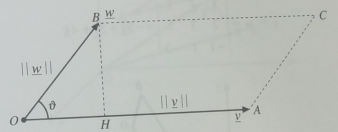
\includegraphics{parallelogramma-vettoriale}
\centering
\end{figure}

Inanzitutto
$$ ||\vec{v} \wedge \vec{w}|| = ||\vec{v}||\cdot ||\vec{w}|| \cdot \sin(\theta) $$

Visto che
$$||\vec{w}|| \cdot \sin(\alpha) = BH$$ allora $$||v \wedge w|| = ||v|| \cdot ||w|| \cdot \sin(\theta) = OA \cdot BH$$ cioè il modulo del prodotto vettoriale corrisponde all'area del parallelogramma $OACB$.

\section{Prodotto Misto}

\begin{definition}
Presi
$$\vec{v} = (a,b,c) = a\vec{i}+b\vec{j}+c\vec{k}$$
$$\vec{w} = (a_1,b_1,c_1) = a_1\vec{i}+b_1\vec{j}+c_1\vec{k}$$
$$\vec{u} = (a_2,b_2,c_2) = a_2\vec{i}+b_2\vec{j}+c_2\vec{k}$$

Definiamo prodotto misto dei tre vettori $\vec{v}, \vec{w},\vec{u}$ il numero
$$v \circ (w \wedge u)$$
\end{definition}

Questo numero è equivalente a il determinante di:
$$
v \circ (w \wedge u) =
\begin{vmatrix}
    a       & b       & c       \\
    a_1     & b_1     & c_1     \\
    a_2     & b_2     & c_2     \\
\end{vmatrix}
$$

\subsection{Proprietà}
\begin{property}
Il prodotto misto è 0 se 3 vettori sono complanari.
\end{property}

Infatti
\begin{property}
Se almeno due di questi vettori sono paralleli, allora due righe sono proporzionali, quindi il determinante della matrice è 0.
\end{property}

\begin{property}
Se i tre vettori non sono paralleli esistono costanti $\alpha, \beta \in \R$ tali che $v = \alpha w + \beta u$, cioè una riga è combinazione lineare delle altre; quindi il determinante della matrice è 0.
\end{property}

\subsection{Significato Geometrico}

\begin{figure}[H]
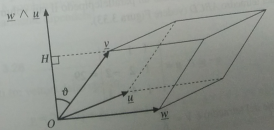
\includegraphics{prodotto-misto}
\centering
\end{figure}

Il modulo del prodotto misto rappresenta il volume del parallelepipedo individuato dai vettori $w, u, v$.

%\section{Combinazioni Lineari}

\section{Dipendenza Lineare}

\begin{definition}
I vettori $v_1, v_2, \ldots, v_n$  si dicono linearmente dipendenti se esistono dei $k_n$ non tutti nulli per cui $$k_1 \cdot v_1 + k_2 \cdot v_2 + \cdots + k_v v_n = 0$$
\end{definition}

\begin{definition}[Combinazione Lineare]
    Si dice che un vettore $v$ è combinazione lineare dei vettori $v_1, \ldots, v_n$ se esistono $a_1,a_2,\ldots,a_n$ tali che
    $$ v = a_1v_1 + \ldots + a_nv_n$$
\end{definition}

\begin{property}
Dei vettori sono linearmente dipendenti solo se almeno uno è combinazione lineare degli altri.
\end{property}


\begin{property}
Due vettori del piano o dello spazio sono linearmente dipendenti se e solo se sono paralleli.
\end{property}

\begin{property}
Tre vettori dello spazio sono linearmente dipendenti se e solo se sono complanari.
\end{property}

\begin{theorem}
Siano dati tre vettori non complanari dello spazio, allora ogni altro vettore dello spazio è combinazione lineare degli altri 3.
\end{theorem}

\begin{definition}
Dei vettori formano una base se non sono linearmente indipendenti, quindi non complanari.
\end{definition}

\begin{property}
$s$ vettori in uno spazio $r$-dimensionale, con $s>r$, sono sempre linearmente dipendenti.
\end{property}


\section{Spazi vettoriali}

\begin{definition}[Spazio vettoriale]
Sia $V$ un insieme di elementi. Definiamo su questo insieme due operazioni, una di addizione e una di moltiplicazione per uno scalare. Valgono inoltre le seguenti proprietà:
\begin{itemize}
\item commutativa
\item associativa
\item esistenza di un elemento nullo (vettore nullo, 0)
\item esistenza di un opposto per ogni elemento
\item $(\alpha\beta)v = \alpha(\beta(v))$
\item $(\alpha\beta)v = \alpha(\beta(v))$
\item $(\alpha+\beta)v = \alpha v + \beta v)$
\item $1 \cdot v = v$
\end{itemize}
Diciamo allora che $V$ è uno spazio vettoriale su $\R$ e chiameremo i suoi elementi vettori.
\end{definition}

\subsection{Sottospazi vettoriali}

\begin{definition}
Sia $V$ uno spazio vettoriale e $S$ un sottoinsieme non vuoto di $V$, si dice che $S$ è un sottospazio di $V$ se valgono le seguenti proprietà:
\begin{itemize}
\item se $u,v \in S$ allora $u+v \in S$
\item se $u \in S$ allora $\alpha u \in S$
\end{itemize}
\end{definition}

\begin{example}
In ogni spazio $V$, ${0}$ e $V$ stesso sono sottospazi. $V$ è sottospazio improprio, ${0}$ è sottospazio banale.
\end{example}


\begin{definition}[Sottospazio generato]
Si dice sottospazio di $V$ generato da $n$ vettori l'inseme di tutte le possibili combinazioni di quegli $n$ vettori.
\end{definition}


\begin{definition}[Base]
Sia $V$ uno spazio vettoriale di dimenione finita; l'insieme dei vettori  $v_1, v_2, \ldots, v_n$ di $V$ è detto una base dello spazio $V$ se questi vettori generano $V$ (cioè ogni elemento di $V$ è combinazione lineare di $v_1, v_2, \ldots, v_n$) e sono linearmente indipendenti.
\end{definition}

\chapter{Geometria Analitica}

\section{Retta nel piano}

\subsection{Equazione della retta}

Supponiamo di avere un vettore $v = (l,m)$ non nullo e un punto $P_0 = (x_0,y_0)$ del piano. Vogliamo determinare tutti i punti $P$ appartentendi alla retta $r$, passante per il punto $P_0$ e parallela al vettore $v$.

\begin{figure}[H]
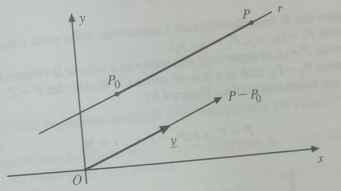
\includegraphics{equazione-retta}
\centering
\end{figure}

Ovviamente il punto $P$ che cerchiamo (generalizzando al caso specifico di un punto solo) appartiene alla retta $r$ se e solo se il vettore $P-P_0$ è parallelo al vettore $\vec{v}$, cioè se esiste una $t$ tale che $P-P_0=t\vec{v}$.

Visto che $P=(x,y)$ e $P_0=(x_0,y_0)$ e $v = (l,m)$ possiamo scrivere
$$
\begin{cases}
x = x_0 + lt \\
y = y_0 + mt
\end{cases}
$$
Che è l'equazione parametrica della retta $r$ passante per il punto $P_0$ e parallela al vettore $\vec{v}$.

\subsection{Retta tra due punti}

Supponiamo di voler determinare l'equazione della retta $r$ passante per due punti distinti $P_1=(x_1,y_1)$, $P_2=(x_2,y_2)$.

Un punto $P=(x,y)$ appartiene a $r$ se e soloe se il vettore $P-P_1$ è parallelo al vettore $P_2-P_1$. Cioè solo se esiste $t  \in \mathbb{R}$ tale che $P-P_1=t(P_2-P_1)$. Da questo otteniamo $$P = P_1+t(P_2-P_1)$$.

Sostituendo le coordinate di $P_1$, $P_2$ e $P$ nell'espressione precedente della retta $r$ si ottiene la seguente

$$
r=
\begin{cases}
x = x_1 + t(x_2-x_1) \\
y = y_1 + t(y_2-y_1)
\end{cases}
$$

Al variare di $t$ si ottengono tutti i punti della retta $r$ passante per $P_1,P_2$.

Al variare di $t \in [0,1]$ si ottengono tutti i punti della retta $r$ passante appartenenti al segmento $P_1P_2$.

E' possibile ricavare $t$ in questo modo:
$$ t = \frac{x-x_1}{x_2-x_1} = \frac{y-y_1}{y_2-y_1}$$


\begin{definition}
L'equzione normale della retta passante per $P_1,P_2$ è: $$\frac{x-x_1}{x_2-x_1} = \frac{y-y_1}{y_2-y_1}$$
\end{definition}

Se $x_2 - x_1=0$ o $y_2 - y_1=0$ allora l'equazione diventa
$$x-x_1 = 0 \text{se} x_2 = x_1$$
$$y-y_1 = 0 \text{se} y_2 = y_1$$

\subsection{Equazione Cartesiana}

\subsubsection{Per due punti}

Dall'equazione normale si ottiene che
$$(x-x_1)(y_2-y_1) = (y-y_1)(x_2-x_1)$$
cioè
$$x(y_2-y_1)-y(x_2-x_1)+y_1x_2-y_2x_1=0$$


\subsubsection{Perpendicolare ad un vettore}

Vogliamo trovare l'equazione della retta $r$ passante per $P_0$ e perpendicolare al vettore $n=(a,b)$.

Cioè se $(P-P_0)\cdot n = 0$.

cioè $$a(x-x_0)+b(y-y_0) = 0$$

\subsection{Parallelismo tra rette}

Date due rette $r$ e $r_1$ di equazioni $ax+by+c=0$ e $a_1x+b_1y+c_1=0$, esse sono parallele se e solo se i vettori $n  = (a,b)$ e $n_1 = (a_1,b_1)$, direttori delle rette, sono paralleli, cioè se eiste un $k$ tale per cui $kn = n_1$.


\subsection{Perpendicolarità tra rette}

Date due rette $r$ e $r_1$ di equazioni $ax+by+c=0$ e $a_1x+b_1y+c_1=0$, esse sono parallele se e solo se il prodotto scalare dei vettori $n  = (a,b)$ e $n_1 = (a_1,b_1)$, direttori delle rette, è nullo.

$$aa_1+bb_1 = 0$$

\subsection{Angolo tra due rette}

Date

$$
r = \begin{cases}
x = x_0 + lt \\
y = y_0 + mt
\end{cases}
$$

$$
r_1 = \begin{cases}
x = x_1 + l_1t \\
y = y_1 + m_1t
\end{cases}
$$

l'angolo tra le rette $r,r_1$ è uguale all'angolo tra i vettori $v_r$ e $v_{r_1}$, cioè

$$\arccos(\pm (v_r \cdot v_{r_1}))$$

\subsection{Equazione in forma esplicita}

Sia data la retta $r$ di equazione $ax+by+c=0$. Supponiamo che sia $b \neq 0$, allora
$$y = -\frac{a}{b} x - \frac{c}{b}$$
Ponendo $m= -\frac{a}{b}$ e $q = -\frac{c}{b}$ si ottiene $y=mx+q$.

Questa formula fornisce l'equazione di tutte le rette del piano, eccetto le rette x=k, parallele all'asse y.

$m$ è detto il coefficiente angolare della reta.

Ponendo $x=t$

$$
\begin{cases}
x= t \\
y=q+mt
\end{cases}
$$

Inoltre
$m = \tan(\theta)$


\subsection{Distanza punto - retta}

Siano dati nel piano una retta $r$ di equazione $ax+by+c=0$ e un punto $P = (x_0,y_0)$.

Sia $H$ il piede della perpendicolare lla retta $r$ condotta da $P_0$.

La misura del segmento $P_0H$ ovvero il numero $\gamma = ||P_0-H||$ è la distanza del punto $P_0$ dalla retta $r$.

Poichè $H \in r$ allora $ax_H+by_h+c=0$.

$P_0-H$ è un vettore parallelo a $v=(a,b)$ (perpendicolare alla retta $r$), quindi $$|(P_0-H) \cdot v| = ||(P_0-H)||||v||$$

cioè

$$\gamma = ||P_0-H|| = \frac{|(P_0-H)\cdot \vec{v}|}{||\vec{v}||}$$

che alla fine è

$$\gamma = \frac{|ax+by_0+c|}{\sqrt{a^2+b^2}}$$

\subsubsection{Distanza rette parallele}

$$\gamma = \frac{|-c_1 + c|}{\sqrt{a2+b^2}}$$

\section{Retta nello spazio}

\subsection{Equazione parametrica}

Preso un punto $P_0$ nello spazio  e un vettore non nullo $v$. Un punto $P$ appartienee alla retta $r$ passante per $P_0$ e parallela a $v$ se e solo se il vettore $P-P_0$ è parallelo al vettore $v$, ossia se e solo se esiste $t \in R$ tale che $$P-P_0=tv$$

$$
\begin{cases}
x = x_0 + lt \\
y = y_0 + mt
z = z_0 + nt
\end{cases}
$$

\subsection{Retta tra due punti}

Come nel piano ma con un punto in più$\ldots$

\section{Piano}

\begin{figure}[H]
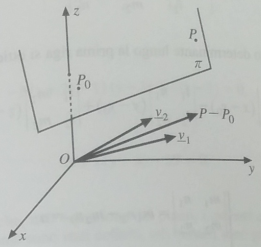
\includegraphics{piano}
\centering
\end{figure}

Dato un punto $P_0$ e due vettori non paralleli dello spazio $v_1=l_1i+m_1j+n_1k$ e $v_2=l_2i+m_2j+n_2k$

Un punto $P$ appartiene al piano  $\pi$ passante per $P_0$ e parallelo ai vettori $v_1$ e $v_2$ se e sole se il vettore $P-P_0$ è complanare con i vettori $v_1$ e $v_2$ ovvero se e solo se esistono $\alpha, \beta \in \mathbb{R}$ tai che $$P-P_0 = \alpha v_1 + \beta v_2$$

Da qui otteniamo l'equazione parametrica del piano

$$
\begin{cases}
x = x_0 + \alpha l_1 + \beta l_2 \\
y = y_0 + \alpha m_1 + \beta m_2 \\
z = z_0 + \alpha n_1 + \beta n_2
\end{cases}
$$

\subsection{Appartenenza al piano}

Consideriamo la seguente matrice

$$
\begin{matrix}
x-x_0 & y-y_0 & z-z_0 \\
l_1 & m_1 & n_1 \\
l_2 & m_2 & n_2
\end{matrix}
$$

La prima riga è combinazione lineare delle altre due, quindi il determinante è uguale a zero.

Un punto $P$ appartiene al piano se e solo se il determinante della matrice è uguale a 0.

Cioè

$$
\begin{vmatrix}
m_1 & n_1 \\
m_2 & n_2 \\
\end{vmatrix}
(x-x_0)
-
\begin{vmatrix}
l_1 & n_1 \\
l_2 & n_2 \\
\end{vmatrix}
(y-y_0)
+
\begin{vmatrix}
l_1 & m_1 \\
l_2 & m_2 \\
\end{vmatrix}
(z-z_0) = 0
$$

Ponendo

$$
\begin{cases}
\begin{vmatrix}
m_1 & n_1 \\
m_2 & n_2 \\
\end{vmatrix} = a \\
- \begin{vmatrix}
l_1 & n_1 \\
l_2 & n_2 \\
\end{vmatrix} = b \\
\begin{vmatrix}
l_1 & m_1 \\
l_2 & m_2 \\
\end{vmatrix} = c
\end{cases}
$$

si ottiene l'equazione di tutti i piani passanti per $P_0$.
$$
a(x-x_0) + b(y-y_0) + c(z-z_0) = 0
$$

\subsection{Equazione piano alternativa}

Siano dati un punto $P_0$ dello spazio e un vettore $u$.

Un punto $P$ appartiene al piano passante per $P_0$ e perpendicolare a $u$ se e solo se il vettore $P-P_0$ è perpendicolare a $u$, cioè $$(P-P_0) \cdot u =0$$

Poichè $P-P_0 = (x-x_0)i + (y-y_0)j +(z-z_0)k$ allora $$ a(x-x_0) + b(y-y_0) +c(z-z_0) = 0$$

\subsection{Piano per tre punti}

Se
$$
\begin{vmatrix}
P_{generico} - P_1
P_2 - P_1
p_3 - P_1
\end{vmatrix} = 0
$$

\subsection{Parallelismo e perpendicolarità tra piani}

Due piani sono paralleli se e solo se i vettori $u$ $u_1$, perpendicolari al piano, sono paralleli, cioè se e solo se esiste $k \in R$ tale che $$u = k u_1$$.


\subsection{Perpendicolarità tra piani}

Due piani sono paralleli se e solo se i vettori $u$ $u_1$, perpendicolari al piano, sono paralleli, cioè se e solo se il loro prodotto scalare è 0.

\subsection{Intersezione di due piani}

Quando due piani si intersecano danno origine ad una retta.

$$
r =
\begin{cases}
a_1x+b_1y+c_1z+d_1 = 0 \\
a_2x+b_2y+c_2z+d_2 = 0 \\
\end{cases}
$$

\subsection{Fasci di piani}

Esisono infiniti piani che passano per una retta $r$. L'insieme di tutti questi piani si chiama fascio di piani di asse $r$.

Se

$$
r =
\begin{cases}
a_1x+b_1y+c_1z+d_1 = 0 \\
a_2x+b_2y+c_2z+d_2 = 0 \\
\end{cases}
$$

allora il fascio di piani individuato è dato da

$$
\lambda(a_1x+b_1y+c_1z+d_1) + \mu (a_2x+b_2y+c_2z+d_2) = 0
$$


\subsection{Parallelismo e perpendicolarità tra una retta e un piano}

\subsubsection{Parallelismo}

\begin{figure}[H]
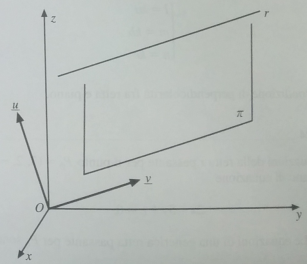
\includegraphics{parallelismo-piano-retta}
\centering
\end{figure}

Il prodotto scalare dei due vettori direttori deve essere 0.

\subsubsection{Perpendicolarità}

\begin{figure}[H]
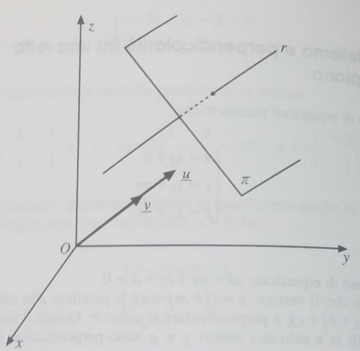
\includegraphics{perpendicolarita-piano-retta}
\centering
\end{figure}

I due vettori direttori devono essere proporzionali.


\subsection{Angolo tra due piani}

E' l'angolo tra i due vettori direttori normali ai due piani.

$$\cos(\alpha) = \frac{|a \cdot b|}{||a|||b||}$$


\subsection{Angolo tra una retta e un piano}

\begin{figure}[H]
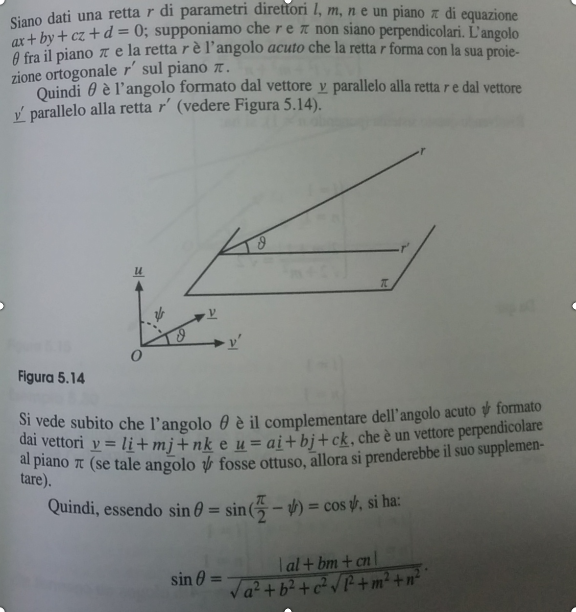
\includegraphics{angolo-retta-piano7}
\centering
\end{figure}

\subsection{Rette sghembe}
Due rette si dicono sghembe se non sono complanari, quindi nè incidenti nè parallele.

Quindi il sistema associato non ha soluzione e i vettori direttori non sono proporzionali.
\chapter{Equazioni differenziali}

Le equazioni differenziali sono equazioni in cui l'incognita è una funzione e in cui sono presenti una o più derivate della funzione incognita.

Ad esempio $f'(x) + f(x) = x$. Cioè tutte le funzioni che sommate alla propria derivata primma danno come risultato $x$

\begin{definition}[Ordine]
Il massimo ordine di derivazione che compare in un' equazione differenziale.
\end{definition}

\begin{example}
$f'(x) = x$

Quali sono le funzioni la cui derivata prima è $x$?

Tutte le funzioni $\frac{x^2}{2} + c = \int x \dif x$
\end{example}

\section{Tipologie e metodi risolutivi}

\subsection{Equazioni differenziali elementari}

In questi casi basta integrare $n$ volte, dove $n$ è l'ordine dell'equazione differenziale.

\begin{example}
$$
y' = 3e^{2x} \to
y = \int 3e^{2x} \dif x \to
y = \frac{3}{2} e^{2x} + c
$$
\end{example}

\begin{example}
$$
y'' = 2-\cos(x) \to
y' = \int 2-\cos(x) \dif x \to
y' = 2x-\sin(x) + c \to
y = \int 2x-\sin(x) + c_1 \dif x \to
y = x^2-\cos(x) + c_1x + c
$$
\end{example}

\subsection{Equazioni differenziali a variabili separabili}

$$y' = f(x) \cdot g(y)$$

Per risolverle:

\begin{enumerate}
\item Separare le variabili
\item Integrare ciascun membro
\item Ricavare y(x)
\end{enumerate}

\begin{example}
$$
y' = y^2 \ln(x) \\
\frac{\dif y}{\dif x} = y^2 \ln(x)  to
\frac{\dif y}{y^2} = \ln(x) \dif x
$$
Posso spezzare $\dif x$ e $\dif y$.

Ora integro.

$$
\int \frac{\dif y}{y^2} = \int \ln(x) \dif x \to
\frac{-1}{y} = x \ln(x) + c
$$

Esplicito la $y$

$$y(x)  = \frac{1}{x\ln(x)-x+c}$$
\end{example}

Se trovo un $t$ tale che $g(t) = 0$ allora $y(x) = t$ è anche soluzione.

\subsection{Equazioni differenziali lineari}

Vediamo per ora quelle del primo ordine, cioè nella forma:

$$y'(x) + a(x)y(x) = f(x)$$

Come procedere:

\begin{enumerate}
\item Calcolare la primitiva di $a(x) = A(x)$
\item Moltiplico entrambi i membri per $e^A(x)$. Quindi a sinistra ho $[y(x)e^{A(x)}]'$
\item Integro entrambi i membri. $y(x)e^{A(x)} = \int f(x)e^{A(x)} \dif x +c$
\item Moltiplico sia a destra che a sinistra per $e^{-A(x)}$. Ottengo $y(x) = e^{-A(x)} \int f(x)e^{A(x)} \dif x +c$
\end{enumerate}

\begin{example}
$$y'(x)-xy(x)=2x$$
$a(x) = -x$, $f(x) = 2x$

Calcolo $\int a(x) = \frac{-x^2}{2}$ 1

Moltiplico tutto per $e^{\frac{-x^2}{2}}$

Ottengo quindi

$$y(x)\cdot e^{\frac{-x^2}{2}} = \int 2x \cdot e^{\frac{-x^2}{2}} \dif x + c$$

Moltiplico per $e^{-A(x)}$.

Ottengo $$y(x) = -2+c\cdot e^{\frac{x^2}{2}}$$
\end{example}

\begin{definition}[Soluzione generale]
$$
y(x) = e^{-A(x)} \int f(x) e^{A(x)} \dif x + c \cdot e^{-A(x)}
$$
\end{definition}

\section{Problema di Cauchy}

Un sistema del tipo
$$
\begin{cases}
\text{Equazione differenziale} \\
\text{Condizioni iniziali}
\end{cases}
$$

\begin{example}
$$
\begin{cases}
y' = -e^{-x} \\
y(0) = 3
\end{cases}
$$
$$
y = e^{-x} + c
$$
Quindi sostituisco $y=f(x)$ e $x=0$
$$
3 = e^{-0} + c \to
c = 2
$$

Quindi $y(x)=e^{-x}+2$ è la soluzione al problema di Cauchy.
\end{example}

\subsection{Esistenza ed unicità della soluzione}

Supponiamo di avere il seguente problema di Cauchy

$$
\begin{cases}
y' = f(x,y) \\
g(x_0) = y_0
\end{cases}
$$
Allora:
\begin{itemize}
\item Se $f(x,y)$ è continua allora esiste almeno una soluzione.
\item Se $f_y(x,y)$ è continua allora esiste una ed una sola soluzione.
\end{itemize}
\chapter{Funzioni a due variabili}

\section{Insieme aperti e chiusi}

\begin{definition}[Insieme aperto]
Un insieme $A$ è aperto se per ogni $x \in A$ (ed un $r>0$) esiste l'intorno $B_r(x) \subseteq A$.
\end{definition}

\begin{example}[Insieme aperto]
$x^2+y^2<1$
\end{example}

\begin{definition}[Insieme chiuso]
Un insieme è chiuso se è il complementare di un insieme aperto.
\end{definition}

\begin{example}[Insieme chiuso]
$x^2+y^2>=1$
\end{example}

\section{Generalità}

\section{Limiti}

Diciamo che $\lim_{(x,y)\to(a,b)} f(x,y) = L$ se:
\begin{itemize}
\item ogni intorno di $(a,b)$ contenga altri punti del dominio di $f$, differenti da $(a,b)$
\item per ogni numero positivo $\epsilon$ esiste un numero positivo $\gamma(\epsilon)$ tale che $|f(x,y)-L|<\epsilon$ vale ogni volta che $(x,y)$ è nel dominio di $f$ e soddisfa $0<\sqrt{(x-a)^2+(y-b)^2}<\gamma$
\end{itemize}

\subsection{Proprietà dei limiti}
Sia $\lim_{(x,y)\to(a,b)} f(x,y) = L$ e $\lim_{(x,y)\to(a,b)} g(x,y) = M$. Valgono allora le seguenti proprietà:
\begin{itemize}
\item Se il limite esiste, esso è unico.
\item $\lim_{(x,y)\to(a,b)} f(x,y) \pm g(x,y) = L \pm M$
\item $\lim_{(x,y)\to(a,b)} f(x,y) g(x,y) = LM$
\item $\lim_{(x,y)\to(a,b)} \frac{f(x,y)}{g(x,y)} = \frac{L}{M}$ purché 
\end{itemize}
\section{Continuità}

Una funzione $f(x,y)$ si dice continua in un punto $(x_0,y_0)$ se:

\begin{itemize}
\item È definita in $(x_0,y_0)$
\item Esiste il limite $\lim_{(x,y)\to(x_0,y_0)} f(x,y)$ ed è uguale a $f(x_0,y_0)$
\end{itemize}

Quindi non è detto che se esiste il limite di una funzione in un punto allora la funzione è definita in quel punto.

\section{Derivabilità}

\subsection{Derivata in $\R$}

$$f'(x_0)=\lim_{h\to 0}\frac{f(x_0+h)-f(x_0)}{h}$$

\subsection{Derivate Parziali}

Calcolate solo rispetto all'asse $x$ o all'asse $y$.

\begin{figure}[H]
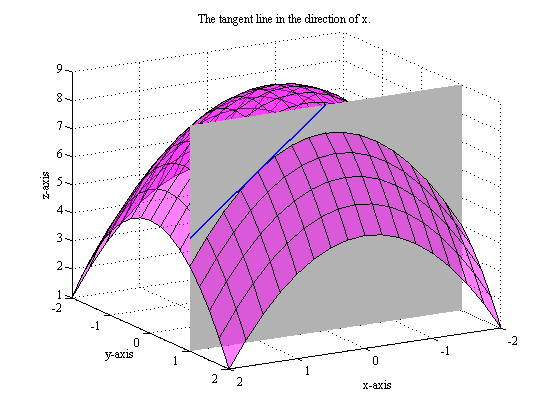
\includegraphics[width=\textwidth]{diff_partial.png}
\end{figure}

Limite di un quoziente di Newton rispetto a una delle due variabili.

$$
f_x(x_0,y_0) = \lim_{h\to 0} \frac{f(x_0+h,y_0)-f(x_0,y_0)}{h}
$$

$$
f_y(x_0,y_0) = \lim_{k\to 0} \frac{f(x_0,y_0+k)-f(x_0,y_0)}{k}
$$

\subsection{Derivata direzionale}

Ci forniscono la rapidità di variazione di $f(x,y)$ lungo una generica direzione $(a,b)$.

Calcolata rispetto ad una qualsiasi retta/direzione.

Fissato un qualunque versore $v=(v_1,v_2)$ posso calcolare:

$$
f_v(a,b) = \lim_{h\to 0^+} \frac{f(a+v_1h,b+v_2h)-f(a,b)}{h}
$$

La derivata direzionale è anche uguale a $$\nabla f(a,b)\circ V$$

\subsection{Sviluppo di Taylor}

Rappresenta la migliore funzione polinomiale di grado $n$ che approssima la funzione $f$ in un intorno di $(x_0, y_0)$.

\begin{multline*}
f(x,y) = f(x_0,y_0)+f_x(x_0,y_0)(x-x_0)+f_y(x_0,y_0)(y-y_0)+ \\ \frac{1}{2} [f_{xx}(x_0,y_0)(x-x_0)^2+2f_{xy}(x_0,y_0)(x-x_0)(y-y_0)+f_{yy}(x_0,y_0)(y-y0)^2]+ \\ o((x-x_0)^2+(y-y_0)^2)
\end{multline*}

\section{Piano tangente}

\subsection{Vettore normale in un punto}

$$n = f_x(a,b)i+f_y(a,b)j-k$$

\subsection{Piano tangente}

Il piano tangente che passa per $P = (a,b,f(a,b))$ è $$f_x(a,b)(x-a)+f_y(a,b)(y-b)-(z-f(a,b))=0$$ cioè
$$z = f(a,b) + f_x(a,b)(x-a) + f_y(a,b)(y-b)$$

\section{Linearizzazione}

\subsection{In $\R$}

La retta tangente al grafico $y=f(x)$ nel punto $x=a$ fornisce un' approssimazione dei valori di $f(x)$ per $x$ vicino ad $a$

$$f(x) \sim L(x) = f(a) + f'(a)(x-a)$$

\subsection{In $\R^2$}

Il piano tangente al grafico di $z = f(x,y)$ in $(a,b)$ è $z = L(x,y)$ dove $$L(x,y) = f(a,b) + f_x(a,b)(x-a) + f_y(a,b)(y-b)$$ è la linearizzazione di $f(x,y)$ in $(a,b)$. La funzione $L(x,y)$ può essere usata per approssimare i valori di $f(x,y)$ vicino a $(a,b)$:
$$
f(x,y) \sim L(x,y) = f(a,b) + f_x(a,b)(x-a) + f_y(a,b)(y-b)
$$
\section{Differenziabilità}

\subsection{Differenziabilità in $\R$}

Una funzione $f$ è differenziabile in $x_0$ se esiste un numero $\alpha \in \R$ tale che:

$$f(x_0+h)=f(x_0)+\alpha h + o(h)$$

per $h \to 0$.

\subsection{Generalità}

Si dice che la funzione $f(x,y)$ è differenziabile in $(x_0,y_0)$ se vale che:
$$
\lim_{(h,k)\to (0,0)} \frac{f(x_0+h,y_0+k) - f(x_0,y_0) - h A - k B}{\sqrt{h^2+k^2}} = 0
$$
dove $A=f_x(x_0,y_0)$ e $B=f_y(x_0,y_0)$

\subsection{Condizioni per la differenziabilità}

Per essere differenziabile una funzione deve essere continua e deve ammettere derivate parziali in $(a,b)$ lungo ogni direzione $V \in \R^2$ (e quindi anche le derivate parziali).

Una funzione è differenziabile se e solo se la supericie $z=f(x,y)$ ha un piano tangente non verticale in $(a,b)$.

\section{Gradiente}

Chiamiamo $\nabla f(x_0,y_0)$ il gradiente della funzione $f$ calcolato in $(x_0,y_0)$.

$$ \nabla f(x_0,y_0) = (f_x(x_0,y_0),f_y(x_0,y_0))$$

Il vettore gradiente calcolato in un punto è anche detto \textbf{differenziale} della funzione in quel punto.

\subsection{Interpretazione geometrica}

\textbf{Per quali versori di $V$ la derivata direzionale risulta Massima o Minima?}

$$
f_V(x_0)  = |\nabla f(x_0)| \cdot |v| \cdot \cos(\theta)
$$

Visto che stiamo trattando versori allora $|v|=1$.

Quindi è la derivata direzionale è massima per $\cos(\theta)=1 \implies \theta=0$

Quindi è la derivata direzionale è minima per $\cos(\theta)=0 \implies \theta=\pi$

La direzione del gradiente calcolato in un punto indica la retta seguendo la quale si trova il massimo incremento della funzione $f$ nell'intorno del punto in cui è calcolato.

\subsection{Differenziale}

Se le derivate prime esistono, possiamo definire il differenziale: il differenziale di una funzione quantifica la variazione infinitesimale della funzione rispetto ad una variabile indipendente.

\section{Matrice Jacobiana}

La matrice jacobiana di una funzione è la matrice i cui elementi sono le derivate parziali prime della funzione.

La sua importanza è legata al fatto che, nel caso la funzione sia differenziabile, la jacobiana rappresenta la migliore approssimazione lineare della funzione vicino a un punto dato.

Sia $\mathbf{f}: U \rightarrow \R^m$ una funzione definita su un insieme aperto $U$ dello spazio euclideo $\R^n$ . La matrice jacobiana della funzione $J {\mathbf f}$ in $\mathbf x = (x_1, \dots, x_n)$ è la matrice delle derivate parziali prime della funzione calcolate in $\mathbf x$:

$$J \, \mathbf f = \begin{bmatrix} \dfrac{\partial f_1}{\partial x_1} & \cdots & \dfrac{\partial f_1}{\partial x_n} \\ \vdots & \ddots & \vdots \\ \dfrac{\partial f_m}{\partial x_1} & \cdots & \dfrac{\partial f_m}{\partial x_n}  \end{bmatrix}\qquad \operatorname (J \, \mathbf f)_{ij} = \frac{\partial f_i (\mathbf {x})}{\partial x_j} $$

\section{Funzione omogenea}

\begin{definition}
Una funzione $f(x_1, \ldots, x_n)$ è detta positivamente omogenea di grado $k$ se, per ogni punto $(x_1, \ldots, x_n)$ del suo dominio e qualunque numero realte $t>0$ si ha
$$ f(tx_1, \ldots, tx_n) = t^k f(x_1, \ldots, x_n)$$

\subsection{Esempi}

$$f(x,y) = x^2 + xy - y^2$$
$$f(x,y) = \sqrt{x^2 + y^2}$$

\end{definition}

\section{Valori Estremi}

\subsection{Punti a cui prestare attenzione}

\begin{itemize}
\item Punti critici (detti anche stazionari) in cui $\nabla f(a,b) = 0$
\item Punti singolari, punti in cui $\nabla f(a,b)$ non esiste
\item Punti di contorno del dominio di $f$
\end{itemize}

\subsection{Classificazione formale}

Se $(a,b)$ è punto critico allora guardo il segno di
$$\delta f = f(a+h,b+k)-f(a,b)$$

\subsection{Classificazione tramite matrice hessiana}

$$
H(x,y) = \begin{vmatrix}
f_{xx} & f_{xy} \\
f_{yx} & f_{yy}
\end{vmatrix}
$$

Sia $P = (a,b)$ un punto stazionario per $f$. Allora valgono le seguenti:
\begin{itemize}
\item Se $H(a,b)$ è definita positiva, allora $f$ ha un minimo locale in $P$
\item Se $H(a,b)$ è definita negativa, allora $f$ ha un massimo locale in $P$
\item Se $H(a,b)$ è indefinita, allora $f$ ha un punto di sella in $P$
\item Se $H(a,b) = 0$, allora questo test è inconcludente
\end{itemize}
\chapter{Integrali doppi}

\section{Generalità}

$$\iint_A f(x,y) \dif x \dif y$$

$A$ è l'insieme (zona) di integrazione ed è un \textbf{sottoinsieme limitato} del piano.

$f(x,y) : A \to R$ è una funzione limitata. Esiste cioè un $M$ tale che $|f(x,y)| \leq M$ $\forall (x,y) \in A$.

\section{Significato geometrico}

\subsection{In $\R$}

$$\int_a^b f(x) \dif x$$

L'integrale è interpretabile geometricamente come l'area con segno della parte di piano sottesa dalla funzione $f(x)$.

\subsection{In $\R^2$}

$$\iint_A f(x,y) \dif x \dif y$$

Se $f(x,y) \ge 0$ allora l'integrale è il volume della parte di spazio compresa tra il piano $xy$ ed il grafico di $f(x,y)$, limitata dalle \textit{pareti verticali} che si proiettano sul bordo di $A$.

Altrimenti, se $f(x,y)$ ha segno variabile in $A$, ``le parti'' al di sotto del piano $xy$ contano con il segno $-$.

\section{Definizione}

\subsection{Funzioni costanti su un rettangolo}

$A= [a,b] \times [c,d]$

Cioè $A$ è un rettangolo delimitato dai lati $ab$ e $cd$.

$f(x,y) = \lambda$, cioè una costante.

Quindi l'integrale è semplicemente $$\lambda \cdot (b-a) \cdot (d-c)$$ ovvero il volume con segno del parallelepipedo.

\subsection{Funzioni costanti su più rettangoli}

Sia $A$ un'unione disgiunta di rettangoli (intuitivamente come tanti grattacieli uno vicino all'altro).

$f(x,y)$ è costante all'interno di ciascun rettangolo, ma può variare da rettangolo a rettangolo.

$f(x,y) = \lambda_i$ $\forall (x,y) \in Rett_i$.

Quindi l'integrale é $$\sum_{i=1}^{n} \lambda_i \cdot \text{Area}(Rett_i)$$

\subsection{Funzioni non costanti su un rettangolo}

Sia $D$ un rettangolo chiuso, con lati paralleli agli assi, $f(x,y)$ è una funzione qualsiasi definita sul dominio $D$.

Supponiamo che $D$ vari tra $a$ e $b$ sull'asse $x$ e tra $c$ e $d$ sull'asse $y$.

Possiamo quindi partizionare il dominio in dei rettangoli più piccoli, individuando dei punti in questo modo:

$$a = x_0 < x_1 < \ldots < x_{m-1} < x_m = b$$


$$c = y_0 < y_1 < \ldots < y_{n-1} < y_n = d$$

In sostanza si individuano $m \cdot n$ rettangoli $Rett_{ij}$.

L'area di ogni rettangolo è $$\delta A_{ij} = \delta x_i \delta y_1$$

La lunghezza della diagonale è
$$\sqrt{(\delta x_i)^2+(\delta y_i)^2}$$

Scelto un punto arbitrario $(x_{ij},y_{ij})$ in ciascuno dei rettangoli individuiamo la somma di Riemann:
$$R(f,P_{artizione}) = \sum^m_{i=1} \sum^n_{j=1} f(x_{ij},y_{ij}) \delta A_{ij}$$

In sostanza base per altezza di un parallelepipedo.

Facendo il limite
$$\lim_{(n,m) \to (\infty, \infty)} R(f,P_{artizione})$$ otteniamo l'integrale doppio di $f$ su $D$, cioè il volume sopra $D$ e sotto il grafico di $f$.


\section{Funzioni integrabili}

\begin{definition}
Si dice che $f$ è integrabile sul rettangolo $D$ e che ha integrale doppio $$I = \iint_D f(x,y) \dif A$$
se, per ogni numero positivo $\epsilon$, esiste un numero $\gamma(\epsilon)$ tale  che $$R(f,P)-I<\epsilon$$ vale per ogni $P$ di $D$ tale che $|P|<\gamma$ e per tutte le scelte di punti $(x_{ij},y_{ij})$.
\end{definition}

\begin{property}
Se una funzione è continua su $D$ allora è integrabile su $D$. Ovviamente, non è detto che se $f$ è integrabile allora è continua.
\end{property}

\section{Integrali doppi su domini generali}

Potrebbe anche essere necessario calcolare un integrale su un dominio $D$ che non è un rettangolo ma un'area qualunque del piano.


\end{document}
